\documentclass[a4paper,10pt]{article}

\usepackage[english]{babel}
\usepackage[utf8]{inputenc}
\usepackage{graphicx}
\usepackage{amsmath,amssymb}
\usepackage{hyperref, url}
\usepackage{tikz}
\usepackage{caption}
\usepackage{subcaption}


\parindent 0mm
\parskip 3mm

% add your name and student number in parenthesis
\title{T-61.5130 Discrete Models and Search \\ Assignment 1}

\author{Sergio Isidoro (410111)\\
	   \textit{Aalto School of Science} \\ \textit{Department of Information and Computer Science}\\ 	   
       {\tt sergio.isidoro@aalto.fi}}

\begin{document}

\maketitle

\section{The approach}
Since the data seems to be hardly hierarchically structured -- machines divided into Locations, Processes divided into Machines and services, a tree like structure is the first guess for representing the data. \\
Genetic Algorithms use such representations (trees) for the encoding of the problem, so a genetic algorithm approach was tried.

\section{Encoding}
For the encoding a Tree structure was built (fig \ref{fig:enc}), being the links between the machines and the processes the only ones being altered.

\begin{figure} [h!]
	\begin{center}
	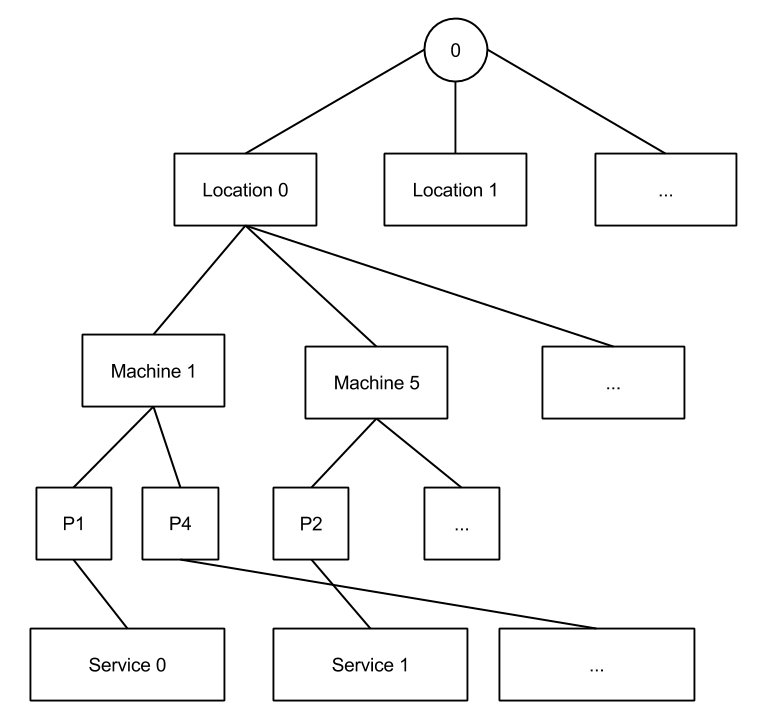
\includegraphics[scale=0.3]{Images/ProblemEncoding.png}
	\caption{Problem Enconding}
    \label{fig:enc}
    \end{center}       
\end{figure}
 
This structures built only once, being reused in the following iterations
 
\section{Selection}
The selection method used was based on the rank of the individuals in a linear form, with a multiplier to emphasize the choosing of the fittest individuals (The used multiplier was 2).

\section{Mutation}
Mutation was done with probability $1/numProcesses$ to assure that at least one attempt to mutate a gene (change a process form one machine to other) would occur. The change is done to a random machine, after being decided that the process is going to "mutate"

\section{Corss Over}
The cross over was done uniformly, with probability defined by a parameter in the main cycle of selection, Cross Over, mutation. Each process has the same probability of being chosen for Cross Over (1/2). A random "mate" is chosen from the individual pool and genes are exchanged - if process is assigned to machine A in one individual, and machine B in other, they will exchange this information. 
\\ By using this we try to assure that the probability of all individuals participating at least once is sufficiently high.

\section{ Notes on Implementation}
The plain mutation of genes was resulting in a overly high percentage of nonviable individuals, so the cross over and mutation of genes would only occur if they resulted in viable offspring. Otherwise mutation of the gene would rollback to original state. - Full viability is not checked on this cases, as it is expensive. Rather, it is kept track of the changes and check if only in the altered regions of the individual are no longer viable  

\subsection{Notes on memory}
Since the selection stage had a bug that took me about 2 days to find (hence the delay on the delivery), memory management is extremely messy (all the variables are replicated in all individuals, representing a huge waste of memory). Careful cleaning of the code will be sufficient. \\
On the other hand, besides the tree, a index of pointers of all processes, services, and machines is kept to improve speed of the program. This is done at high expense of memory. The alternative would be to search the tree for every node, every time. \\
Also a list of "dead" individuals is kept in a list. This could be avoided by "translating" all individuals into their configurations, and reset them during selection stage. The former approach was used because it was simpler to code. 


\end{document}